\chapter{Gesamtsystem}
\label{cha:gesamtsystem}
In diesem Kapitel wird der Systemaufbau und insbesondere die Integration von \emph{CCMail} in dasselbe diskutiert.
Folgendes Diagramm illustriert den Systemaufbau und die Integration von \emph{CCMail} in das Gesamtsystem. 
\\
\begin{figure}[h]
\centering
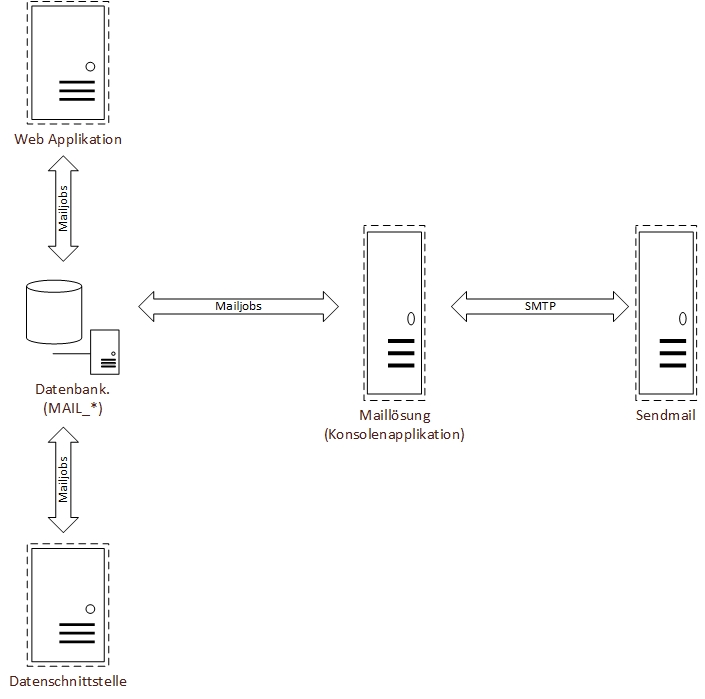
\includegraphics[scale=0.5]{Systemaufbau_alt.jpg} %{CS0031}
\caption{Systemaufbau und Integration von \emph{CCMail}}
\label{fig:ccmail-system-integration}
\end{figure}
\ \newline
Aus diesem Diagramm lässt sich ableiten dass das Kernstück des E-Mail Versandes die Datenbank ist. In der Datenbank werden die zu versendenden E-Mail-Nachrichten als sogenannte \emph{MailJob} in der Datenbank gespeichert und anschließend von \emph{CCMail} ausgelesen und verarbeitet. Ein \emph{MailJob} ist hierbei als eine Entität einer Datenbanktabelle anzusehen.
\newline\newline
\emph{CleverWeb} und \emph{CleverInterface} erstellen über ihre Datenbankzugriffsschicht \emph{MailJob} Entitäten in der Datenbank, welche zeitgesteuert von \emph{CCMail} ausgelesen, verarbeitet und versendet werden. \emph{CCMail} ist als eine Konsolen-Anwendung Implementiert und enthält alle Ressourcen, die es benötigt um die \emph{MailJob} Entitäten zu verarbeiten.

\section{Prozessübersicht}
Im folgenden wird ein Beispiel für den Gesamtprozess diskutiert, also vom Anlegen eines \emph{MailJob} bis hin zum Versand der eigentlichen E-Mail-Nachricht. Als Kernkomponente des E-Mail-Versandes wurde die Datenbank identifiziert, die die \emph{MailJob} Entitäten hält. Dieser Ansatz ist an sich nicht als schlecht anzusehen, jedoch verbirgt sich hier eines der Hauptprobleme des E-Mail-Versandes. Nämlich die Inkonsistenz der versendeten E-Mail-Nachrichten, durch die Zeitdifferenz zwischen dem Anlegen eines \emph{MailJob} und dem tatsächlichen Versand der E-Mail-Nachricht wie in folgendem Sequenz-Diagramm illustriert wird.
\begin{figure}[h]
\centering
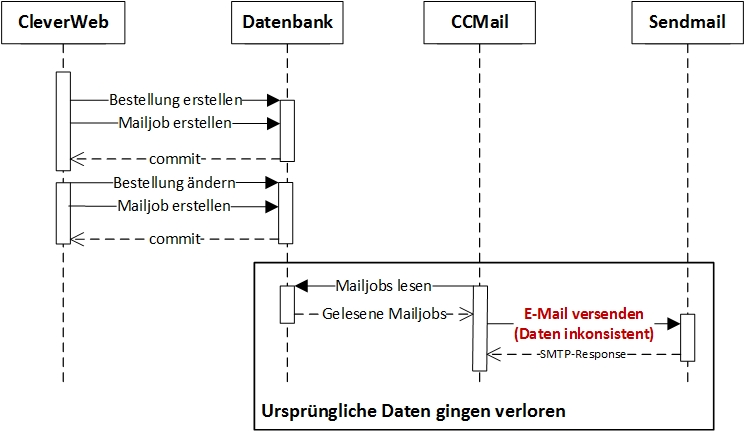
\includegraphics[scale=0.8]{prozess_sequence_emailversand.jpg}
\caption{Beispiel für den Gesamtprozess eines E-Mail Versandes}
\label{fig:sequence-diagram-mail-send}
\end{figure}
\ \newline
Eines der Hauptprobleme an diesem Prozess ist die Inkonsistenz, was in der Art und Weise wie die \emph{MailJob} Entitäten verarbeitet werden begründet ist. Ein \emph{MailJob} hält die Informationen für den Versand einer E-Mail wobei hierbei nicht die gesamte E-Mail-Nachricht gespeichert ist sondern lediglich die Parameter, die in einer Datenbankabfrage genutzt werden um die Daten für die E-Mail-Nachricht zu erhalten. Sollten sich die Datenbank Entitäten der involvierten Tabellen ändern, wie in diesem Beispiel eine Bestellung, so ist dieselbe E-Mail-Nachricht, die bereits versendet wurde nicht mehr wieder herstellbar, da sich die zugrundeliegenden Daten geändert haben.
\newline\newline
Ein Weiteres Problem liegt in der zeitgesteuerten Abarbeitung der \emph{MailJob} Entitäten von \emph{CCMail}. Es wurde lange Zeit nicht geprüft ob bereits ein \emph{CCMail} Prozess gestartet wurde bevor dieser gestartet wird. Dies hat dazu geführt dass es vorkam das mehrere Prozesse gleichzeitig die \emph{MailJob} Entitäten verarbeiten und daher wurden E-Mail-Nachrichten mehrmals versendet. 
\chapter{CCMail}
\label{cha:ccmail}
Nachdem das Gesamtsystem und ein Beispiel für den Prozess eines E-Mail-Versandes diskutiert wurden wird sich nun mit dem Design und der Implementierung von \emph{CCMail} befasst. \emph{CCMail} wurde als Konsolen-Anwendung implementiert und hält alle implementierten E-Mail-Typen, die zur Verfügung stehen wie:
\begin{enumerate}
	\item E-Mail-Vorlagen
	\item Datenbankabfragen
	\item E-Mail-Typ spezifische Implementierungen
\end{enumerate}
\ \newline
Es wurde hierbei eine Klasse namens \emph{CCBasicEmail}
implementiert, die alle nötigen Funktionalitäten für den Versand einer E-Mail-Nachricht enthält, sowie eine Klasse namens \emph{CCMailingDao} die alle Datenbankabfragen über alle E-Mail-Typen hält.
\begin{figure}[h]
\centering
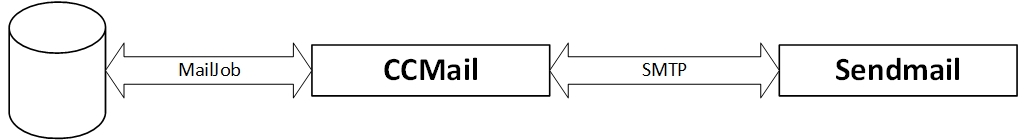
\includegraphics[scale=0.5]{teilsystem_ccmail.jpg} 
\caption{Teilsystem \emph{CCMail}}
\label{fig:class-hierarchie-email}
\end{figure}


\newpage
\section{Klassenhierarchien}
\label{sec:klassen-hierarchien}
Um das Design von \emph{CCMail} zu illustrieren wird im Folgenden näher auf die Klassenhierarchien von \emph{CCMail} eingegangen. Im Grunde besteht \emph{CCMail} aus den beiden folgenden Softwarekomponenten:
\begin{enumerate}
	\item\emph{CCBasicEmail}\newline
	Wurzelklasse aller E-Mail-Typen die als abgeleitete Klassen von \emph{CCBasicEmail} implementiert wurden
	\item\emph{CCMailingDao}\newline
	Schnittstelle zur Datenbank, welche alle Abfragen auf die Datenbank über alle E-Mail-Typen hinweg spezifiziert. 
\end{enumerate}
\ \newline
Die Klassenhierarchien geben einen guten Einblick in das Design und die Struktur von \emph{CCMail} und werden aufzeigen was der Grundgedanke beim Design von \emph{CCMail} war und warum man sich für das Design entschieden hat. 
\subsection{CCBasicEmail}
\label{sec:klassen_hierarchie_ccbasic_mail}
Einleitend betrachten wir die Klassenhierarchie der Klasse \emph{CCBasicEmail}, die die Wurzelklasse aller E-Mail-Typen darstellt.
\begin{figure}[h]
\centering
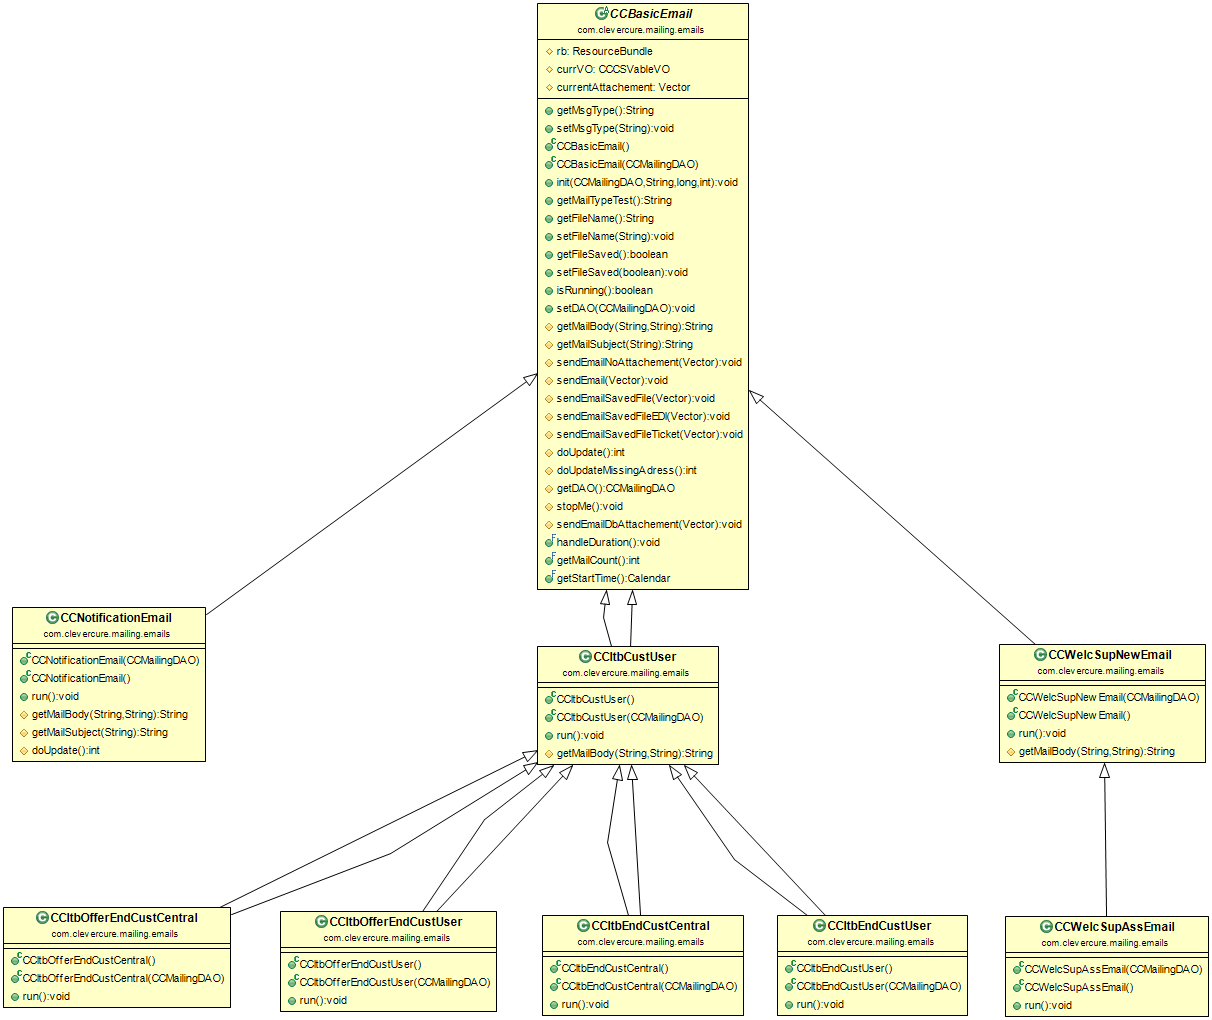
\includegraphics[scale=0.55]{class_diagram_basic_email.png} 
\caption{Auszug aus der Klassenhierarchie von \emph{CCBasicEmail}}
\label{fig:klassen-hierarchie-ccbasicemail}
\end{figure}
\ \newpage
In diesem Klassendiagramm sieht erkennt man sehr gut dass man sich dazu entschieden hat die einzelnen E-Mail-Typen als eigene Klassen abzubilden. Somit ist jeder E-Mail-Typ auch als eigener Java Typ abgebildet. Am Beispiel der Klasse \emph{CCItbCustUser} ist ersichtlich dass neben dem Abbilden eines E-Mail-Typs als eigene Java Klasse man ebenfalls eine eigene Subklassenhierarchie eingeführt hat um E-Mail-Typen, die in einem gemeinsamen Kontext sich befinden zu gruppieren. Ob dies ein guter Ansatz um Kontextabhängige Ressourcen gruppieren ist zu hinterfragen. Es gäbe hier andere Ansätze wie man eine solche Gruppierung hätte realisieren können, die flexible sind als eine Klassenhierarchie. Eine Klassenhierarchie ist an sich starr und nicht flexibel und Änderungen an der Struktur können sich negativ in der Gesamtstruktur auswirken.
\subsection{CCMailingDao}
Im Gegensatz zur Strukturierung der E-Mail-Typen hat man sich bei der Datenzugriffsschicht nicht dazu entschieden diese kontextabhängig zu gruppieren. Hier wurden alle Datenbankabfragen in einer einzigen Schnittstelle spezifiziert ohne Rücksichtnahme auf deren Kontext.
\begin{figure}[h]
\centering
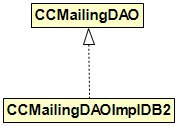
\includegraphics[scale=0.55]{class_diagram_mailing_ao.png} 
\caption{Klassenhierarchie von \emph{CCMailingDao}}
\label{fig:class-hierarchie-ccmailing-dao}
\end{figure}
\ \newline
Diese Klassenhierarchie ist sehr einfach, da man sich nicht für eine Gruppierung entschieden hat. Hier ist zu bemängeln dass sich hier alle Datenbankabfragen über alle E-Mail-Typen hinweg befinden und man es versäumt hat hier Schnittstellen einzuführen, die die kontextabhängigen Datenbankabfragen spezifizieren. Mit einer Aufteilung auf mehrere Schnittstellen hätte man es sich vereinfacht diese die Datenbankabfragen zu warten. Mit diesem Ansatz ist man erstens gezwungen Präfixe für die Methodennamen einzuführen, da Namenskollisionen sehr wahrscheinlich sind und zweitens muss man darauf Acht geben bestehende Implementierungen bei einem Refaktorisieren einer oder mehrerer kontextabhängigen Implementierungen nicht zu verändern. Alle Implementierungen nutzen dieselben Ressourcen und müssen daher auf den kleinsten gemeinsamen Nenner zusammengeführt werden, oder man führt hier wiederum eigene Ressourcen ein, die sich durch ihren Namen unterscheiden.
\newpage
\begin{figure}[h]
\centering
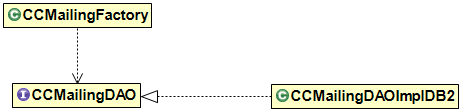
\includegraphics[scale=0.55]{class_diagram_mailing_dao_factory.png} 
\caption{\emph{CCMailingDaoFactory} für \emph{CCMailingDao}}
\label{fig:class-hierarchie-ccbasicemail}
\end{figure}
\ \newline
Zu kritisieren ist hier auch die Art und Weise wie eine Instanz von \emph{CCMailingDao} erzeugt wird. Man nutzt hier den Factory-Pattern, jedoch wird hier statisch die zu verwendende Implementierung in der Factory \emph{CCMailingDaoFactory} definiert was das Austauschen der Implementierung unmöglich macht. Zusätzlich befindet sich die Schnittstelle zusammen mit ihrer Implementierung in ein und demselben Artefakt. Dies ist als ein sehr halbherziger Versuch zu werten die Implementierung austauschbar zu machen.  
\newpage
\section{Implementierung CCItbCustUser}
Nachdem die Klassenhierarchien diskutiert wurden wird im folgenden die Implementierung der Klasse \emph{CCItbCustUser} und dessen Ableitungen diskutiert. Diese Implementierung dient als Beispiel für die restlichen E-Mail-Typ Implementierungen, die nach dem selben Prinzip mit ähnlichen Umfang implementiert wurden. Im Punkt~\ref{sec:klassen_hierarchie_ccbasic_mail} wurde behauptet dass diese Ableitungen eingeführt wurden um E-Mail-Typen zu gruppieren. Man könnte aber auch davon ausgehen dass diese eigene Subklassenhierarchie eingeführt wurde um gemeinsame Funktionalitäten für die abgeleiteten E-Mail-Typen zu kapseln. 
\newline\textbf{STOPPED HERE at 07.12.2015: 20:53}
\begin{program}
\caption{CCItbCustUser E-Mail Typ Implementierung}
\label{CCItbCustUser.java}
\begin{JavaCode}
public class CCItbCustUser extends CCBasicEmail {
	
	private Map cache = new HashMap();

	public CCItbCustUser() {
		super();
	}

	public CCItbCustUser(CCMailingDAO dao) {
		super(dao);
	}

	@Override
	String getMailType() {
		return "ISCU";
	}
	
	@Override
	public void run() {
		try {
			sendEmailNoAttachement(getDAO().getItbStartCustUserMailText());
		} catch (DAOSysException ex) {
			LOG.error("DAOSysException in CCItbCustUser.run: ",
						ex);
		} finally {
			stopMe();
		}
	}
	
	@Override
	protected String getMailBody(String bodyKey, String bodySQLKey)
		throws DAOSysException {
		int lanId = ((CCItbVO)currVO).getLanguageId();
		int itbhId = ((CCItbVO)currVO).getItbhID();
		String body = "";
		String key = itbhId	+ "_" + lanId;
		if (cache.containsKey(key)) {
			body = (String) cache.get(key);
			LOG.debug("48: Got from cache key: " + key 
								+ " body: " + body);
		} else {
			Object [] allParams = getDAO().getItbCustData((CCItbVO)currVO, 19);
			// Message body parameters retrieved from result set for body template
			MessageFormat form = new MessageFormat(rb.getString(bodyKey).trim());
	 		body = form.format(params);
	 		cache.put(key, body);
	 		LOG.debug("48: DB access for the key: " + key
	 						+ " got body: " + body);
		}
		return body;
	}
}
\end{JavaCode}
\end{program}

\newpage
In dieser Implementierung ist gut zu erkennen, dass die einzelnen E-Mail Typen - oder mit anderen Worten - die einzelnen Implementierungen der Basisklasse \emph{BasicEmail} lediglich folgende Funktionalitäten implementieren:
\begin{itemize}
	\item\emph{getMailType()}\\
	Bereitstellen eines eindeutigen Schlüssels, der diesen E-Mail Typ identifiziert.
	\item\emph{getMailBody()}\\
	Erstellen der E-Mail Nachricht aus einer Vorlage, welche mit Parametern - Daten werden aus Datenbank gelesen - befüllt wird.
	\item\emph{run()\\}
	Einstiegspunkt des E-Mail Typs, wo definiert wird welche Art von E-Mail erstellt werden soll. (\emph{BasicEmail} stellt mehrere Methoden zur Verfügung)
\end{itemize}
\ \\

\chapter{Client Implementierung}
\label{cha:client-api}
Da die Kommunikation ausschließlich über die Datenbank erfolgt ist eine echte Client API nicht vorhanden. Alle Systeme implementieren das Erstellen der Mailjob Einträge selbstständig und es wird keine gemeinsame Client API verwendet, was einen gewissen Grad der Inkonsistenz bei Änderungen der Datenstruktur sowie der Semantik der Daten mit sich bringt. Als Beispiel wird hier die Semantik der einzelnen Spalten angeführt, die zwar technisch sich innerhalb einer Datentyp Domain befinden, sich die semantische Bedeutung der enthaltenen Daten aber unterscheidet. Dies ist zwar Teil der Datenbank Integration aber die Tatsache dass diese Semantik rein innerhalb der Applikation abgebildet werden kann und nicht über die Datenbankfunktionalitäten wie z.B.: Fremdschlüssel wird dieser Teil hier diskutiert. Da die Maillösung über SQL Abfragen die Daten für die E-Mail Nachricht erhält müssen auch Parameter bereitgestellt werden, die in der SQL Abfrage gesetzt werden. Diese Parameter wurden \emph{'generisch'} über eine festgesetzte Anzahl von Tabellenspalten abgebildet, dessen enthaltene Daten je nach E-Mailtyp anders interpretiert werden. Es kann also sein das ein Eintrag einer Tabellen für die Spalte \emph{COL\_1} einen String enthält mit dem Wert \emph{'Thomas Herzog'} und ein anderer Eintrag einen string mit dem Wert \emph{'14'} der in der SQL Abfrage aber als Integer Datentyp behandelt wird. Die Systeme die Mailjobs erzeugen müssen sich also dem Kontext einer E-Mail bewusst sein, sowie müssen berücksichtigen, dass die richten Spalten der Tabelle \emph{MAIL\_JOB} mit den richtigen Daten befüllt werden, wobei auch beachtet werden muss in welchen Datentyp der Datensatz in weiterer Folge durch die Mailösung interpretiert wird.\\
Dies ist in meinen Augen sehr inkonsistent und fehleranfällig und hat auch schon einige Probleme verursacht.\\\\
\begin{figure}[h]
\centering
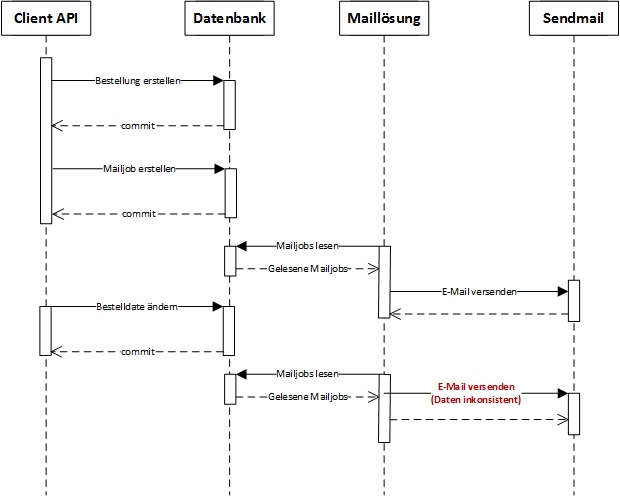
\includegraphics[scale=0.70]{Emailvesand_Client_Api.jpg}
\caption{Diese Abbildung zeigt das Problem der inkonsistenten Daten beim erneuten E-Mailversand einer bereits versendeten E-Mail, mit dem Beispiel einer angelegten und anschließend geänderten Bestellung, auf}
\label{fig:sequence-diagram-mail-send}
\end{figure}
\newpage
